\documentclass[border=16pt]{standalone}
\usepackage[T1]{fontenc}
\usepackage{helvet}
\renewcommand{\familydefault}{\sfdefault}
\usepackage{tikz}
\usetikzlibrary{positioning,arrows.meta,calc,decorations.pathreplacing}

\definecolor{clsBlue}{HTML}{2C5AA0}
\definecolor{ownGreen}{HTML}{1F7A5A}
\definecolor{ownBg}{HTML}{E4F3EC}
\definecolor{viewOr}{HTML}{C4600A}
\definecolor{viewBg}{HTML}{FCEBD7}
\definecolor{structPu}{HTML}{6B3FA0}
\definecolor{structBg}{HTML}{F1EAF9}
\definecolor{dispInk}{HTML}{30357E}
\definecolor{dispBg}{HTML}{E7E8F6}

\begin{document}
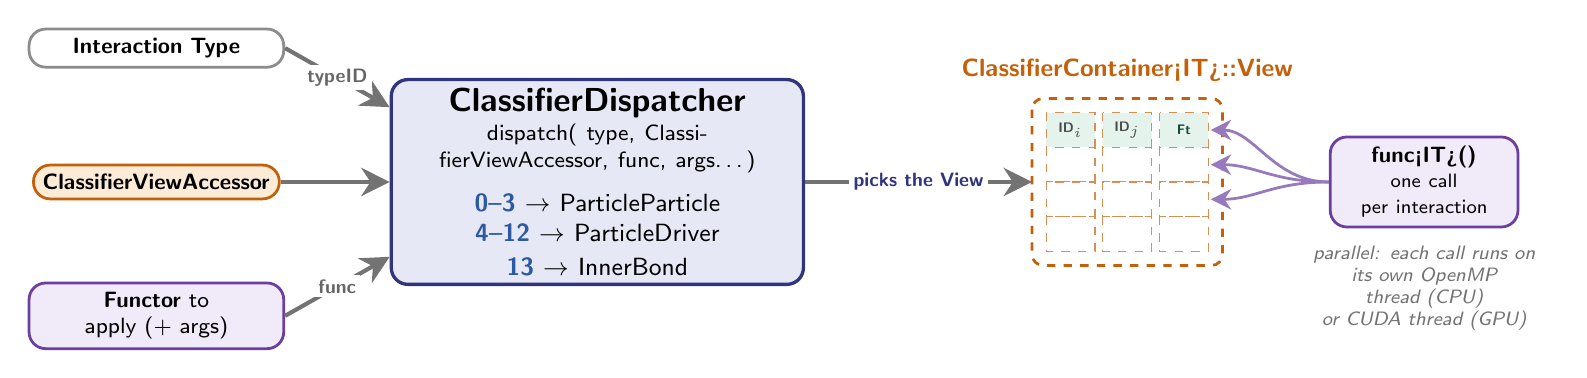
\begin{tikzpicture}[
  font=\sffamily,
  >=Stealth,
  bx/.style={rounded corners=6pt, line width=1pt},
  flow/.style={-{Stealth[length=3.6mm,width=3.6mm]}, line width=1.5pt, draw=black!55},
  small/.style={-{Stealth[length=2.6mm,width=2.6mm]}, line width=1pt, draw=structPu!70},
  plab/.style={font=\sffamily\scriptsize\bfseries, text=black!60, fill=white, inner sep=1.5pt},
]

% =========================== 3 INPUT PARAMETERS ===========================
\node[bx, draw=black!45, fill=white, align=center, font=\sffamily\footnotesize, text width=3.0cm] (pin)
  at (0,1.7){\textbf{Interaction Type}};
\node[bx, draw=viewOr, fill=viewBg, align=center, font=\sffamily\footnotesize] (piva)
  at (0,0.0){\textbf{ClassifierViewAccessor}};
\node[bx, draw=structPu, fill=structBg, align=center, font=\sffamily\footnotesize, text width=3.0cm] (pfun)
  at (0,-1.7){\textbf{Functor} to \\apply (+ args)};

% =========================== DISPATCHER ===========================
\node[bx, draw=dispInk, fill=dispBg, line width=1.2pt, align=center, text width=5.0cm] (disp)
  at (5.6,0){%
  \textbf{\large ClassifierDispatcher}\\[1pt]
  \footnotesize dispatch( type, ClassifierViewAccessor, func, args\dots )\\[5pt]
  \small
  \textcolor{clsBlue}{\textbf{0--3}} $\to$ ParticleParticle\\
  \textcolor{clsBlue}{\textbf{4--12}} $\to$ ParticleDriver\\
  \textcolor{clsBlue}{\textbf{13}} $\to$ InnerBond};

\draw[flow] (pin.east)  -- node[plab]{typeID} ($(disp.west)+(0,0.95)$);
\draw[flow] (piva.east) -- ($(disp.west)+(0,0.0)$);
\draw[flow] (pfun.east) -- node[plab]{func} ($(disp.west)+(0,-0.95)$);

% =========================== SELECTED VIEW ===========================
\def\vcw{0.62}\def\vch{0.44}\def\vcg{0.10}
\def\vx{11.3}\def\vy{0.88}
\foreach \c in {0,1,2}{
  \pgfmathsetmacro\xx{\vx+\c*(\vcw+\vcg)}
  \foreach \r in {0,1,2,3}{
    \pgfmathsetmacro\yy{\vy-\r*\vch}
    \ifnum\r=0 \def\cb{ownBg}\else \def\cb{white}\fi
    \fill[\cb,draw=viewOr!70,dashed,line width=0.4pt] ({\xx},{\yy}) rectangle ({\xx+\vcw},{\yy-\vch});}}
\node[font=\tiny\bfseries,text=black!70]          at ({\vx+0.5*\vcw},{\vy-0.5*\vch}){ID$_i$};
\node[font=\tiny\bfseries,text=black!70]          at ({\vx+1*(\vcw+\vcg)+0.5*\vcw},{\vy-0.5*\vch}){ID$_j$};
\node[font=\tiny\bfseries,text=ownGreen!60!black] at ({\vx+2*(\vcw+\vcg)+0.5*\vcw},{\vy-0.5*\vch}){Ft};

\coordinate (vTL) at ({\vx-0.18},{\vy+0.18});
\coordinate (vBR) at ({\vx+3*\vcw+2*\vcg+0.18},{\vy-4*\vch-0.18});
\draw[viewOr,dashed,line width=1pt,rounded corners=4pt] (vTL) rectangle (vBR);
\node[font=\sffamily\small\bfseries,text=viewOr,anchor=south] at ({\vx+1.03},{\vy+0.28})
  {ClassifierContainer<IT>::View};


% =========================== FUNCTOR PER INTERACTION ===========================
\node[bx, draw=structPu, fill=structBg, align=center, font=\sffamily\footnotesize, text width=2.15cm] (fcall)
  at (16.1,0.0){\textbf{func<IT>()}\\[1pt]\scriptsize one call\\ per interaction};
\foreach \r in {1,2,3}{
  \draw[small] (fcall.west) .. controls +(-0.7,0) and +(0.55,0) ..
     ({\vx+3*\vcw+2*\vcg+0.03},{\vy-\r*\vch+0.5*\vch});}
\node[font=\sffamily\scriptsize\itshape, text=black!55, align=center, text width=3.2cm] (fcallcapt)
  at (16.1,-1.35){parallel: each call runs on\\ its own OpenMP thread (CPU)\\ or CUDA thread (GPU)};

% dispatcher -> view
\draw[flow] (disp.east) -- node[plab, text=dispInk]{picks the View} ({\vx-0.18},{\vy-2*\vch});

\end{tikzpicture}
\end{document}
